\documentclass[11pt, a4paper]{article}
\usepackage[a4paper, margin=2.5cm]{geometry}
\usepackage[T1]{fontenc}
\usepackage[utf8]{inputenc}
\usepackage{helvet}
\renewcommand{\familydefault}{\sfdefault}
\usepackage{amsmath}
\usepackage{booktabs}
\usepackage{graphicx}
\usepackage[table]{xcolor}
\usepackage{hyperref}

\usepackage{fancyhdr}
\setlength{\headheight}{14pt}
\pagestyle{fancy}
\fancyhf{}
\fancyhead[L]{\small Artificial Intelligence -- Assignment 1}
\fancyhead[R]{\small 8-Puzzle Solver}
\fancyfoot[C]{\small\thepage}
\renewcommand{\headrulewidth}{0.4pt}

\definecolor{primary}{RGB}{0, 80, 160}

\begin{document}

\begin{titlepage}
    \thispagestyle{fancy}
    \centering
    \vspace*{4cm}
    {\Huge\color{primary}\textbf{Assignment 1: 8-Puzzle Solver}\par}
    \vspace{1.5cm}
    {\Large\textbf{Artificial Intelligence}\par}
    \vspace{0.5cm}
    {\large Computer and Systems Program\par}
    \vspace{3cm}
    \textbf{Submitted by:}\par
    \vspace{0.8cm}
    {\Large
    \begin{tabular}{ll}
        \textbf{Name} & \textbf{ID} \\
        \midrule
        Abdullah Ahmed Elsherbiny & 24010411 \\
        \addlinespace
        Youssef Diaa Elghanam & 24010851 \\
    \end{tabular}
    }\par
    \vfill
    {\large Fall 2026\par}
\end{titlepage}

\section{Overview}
The 8-puzzle is a classic sliding puzzle consisting of a $3 \times 3$ grid with 8 numbered tiles and one blank space (represented by 0). The objective is to transition from a given initial state to the goal state \texttt{(0, 1, 2, 3, 4, 5, 6, 7, 8)} by sliding tiles horizontally or vertically into the blank space. Each move (Up, Down, Left, Right) has a uniform cost of 1.

\section{Data Structures}
To ensure efficiency and memory optimization, the following data structures were utilized across the algorithms:
\begin{itemize}
    \item \textbf{State Representation:} The board is represented as an immutable 1D \texttt{tuple} of 9 integers (e.g., \texttt{(1, 2, 5, 3, 4, 0, 6, 7, 8)}). Tuples are hashable, allowing them to be used as keys in dictionaries and elements in sets for $O(1)$ lookups.
    \item \textbf{Breadth-First Search (BFS):} Utilizes \texttt{collections.deque} for a double-ended queue, providing $O(1)$ time complexity for FIFO operations.
    \item \textbf{Depth-First Search (DFS) \& IDDFS:} Utilize Python lists as LIFO stacks.
    \item \textbf{A$^*$ Search:} Utilizes \texttt{heapq}, a binary heap priority queue, to efficiently pop the node with the lowest $f(n)$ cost.
    \item \textbf{Path Reconstruction \& Cycle Detection:} A \texttt{parent} dictionary maps each visited \texttt{child\_state} to its \texttt{(parent\_state, move)}. This acts as both the ``visited'' set and the path-tracing mechanism, minimizing memory overhead.
\end{itemize}

\section{Search Algorithms Implementation}
The solver implements both uninformed and informed search algorithms:

\subsection{Uninformed Search}
\begin{itemize}
    \item \textbf{Breadth-First Search (BFS):} Expands the shallowest unexpanded node. It guarantees the shortest path (optimal) for this problem since step costs are uniform. However, it requires exponential memory space.
    \item \textbf{Depth-First Search (DFS):} Expands the deepest unexpanded node. It is implemented iteratively to prevent recursion limit errors. While highly memory-efficient, it does not guarantee an optimal path and can generate heavily redundant sequences.
    \item \textbf{Iterative Deepening DFS (IDDFS):} Combines the space efficiency of DFS with the optimality of BFS. It repeatedly runs a depth-limited DFS, incrementing the depth limit until the goal is found. Though it re-generates upper levels, the overhead is minimal compared to the memory savings.
\end{itemize}

\subsection{Informed Search (A$^*$)}
A$^*$ search evaluates nodes by combining $g(n)$, the cost to reach the node, and $h(n)$, the estimated cost to get from the node to the goal: $f(n) = g(n) + h(n)$.

\section{Heuristics and Comparison}
Two heuristics were implemented for A$^*$ search. Both ignore the blank space.

\begin{enumerate}
    \item \textbf{Manhattan Distance:} The sum of the absolute horizontal and vertical grid distances for each tile to its target position.
    \[ h_{manhattan} = \sum_{i=1}^{8} \left( |x_i - x_{goal}| + |y_i - y_{goal}| \right) \]
    \item \textbf{Euclidean Distance:} The straight-line distance for each tile to its target position.
    \[ h_{euclidean} = \sum_{i=1}^{8} \sqrt{(x_i - x_{goal})^2 + (y_i - y_{goal})^2} \]
\end{enumerate}

\noindent\textbf{Admissibility and Dominance:}
Both heuristics are \textit{admissible} because they never overestimate the true cost to reach the goal. A tile can move at most one square per step, meaning it physically cannot reach its goal faster than the Manhattan or Euclidean distance.
However, because diagonal moves are illegal in the 8-puzzle, the Euclidean distance often underestimates the true cost more severely than the Manhattan distance. Mathematically, $h_{euclidean}(n) \le h_{manhattan}(n)$ for all states. Therefore, the \textbf{Manhattan heuristic dominates the Euclidean heuristic}. Because it is more informed (closer to the true cost), A$^*$ with Manhattan distance expands fewer or equal nodes compared to Euclidean distance, making it the superior heuristic for this problem.

\section{Assumptions and Design Details}
\begin{itemize}
    \item \textbf{Solvability Test:} Before executing any search, the algorithm counts the number of \textit{inversions} in the board. If the number of inversions is odd, the 8-puzzle is mathematically unsolvable, and the program safely aborts instead of searching infinitely.
    \item \textbf{Node Expansion Order:} Successors are strictly generated in the order: \textit{Up, Down, Left, Right}. This ensures deterministic and reproducible results.
    \item \textbf{Expansion Metric:} A node is counted as ``expanded'' only when it is popped from the frontier and its children are generated.
\end{itemize}

\section{Extra Work: GUI Visualization}
A complete graphical user interface (GUI) was developed using \texttt{tkinter} (\texttt{gui.py}). This application provides:
\begin{itemize}
    \item Interactive text boxes to input the initial 9-tile configuration.
    \item Real-time animation of the tiles sliding to reach the goal.
    \item A dynamic step-by-step trace table displaying the sequence of moves and queue/stack/heap snapshots at each state.
    \item The ability to fast-forward (skip) the animation to instantly view the final path and metrics.
\end{itemize}

\begin{figure}[htbp]
    \centering
    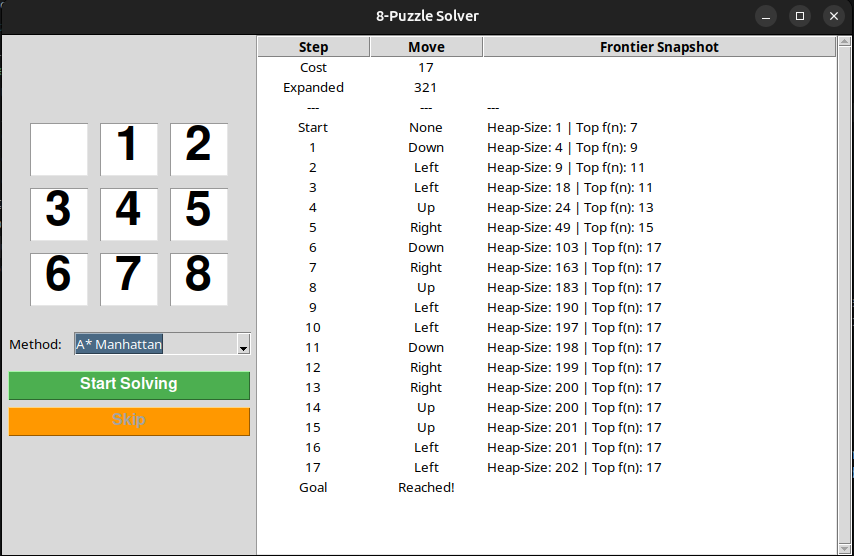
\includegraphics[width=0.85\textwidth, keepaspectratio]{gui.png}
    \caption{8-Puzzle Solver Graphical User Interface}
\end{figure}

\section{Sample Run and Results}
Testing on the initial state \texttt{1, 2, 5, 3, 4, 0, 6, 7, 8}, the initial grid looks like this:
\begin{center}
    1 2 5 \\
    3 4 \_ \\
    6 7 8
\end{center}

\noindent All optimal algorithms find the path: \textbf{Up, Left, Left}. Below is a summary of the performance metrics across the different algorithms for this state:

\vspace{0.5cm}
\begin{center}
\begin{tabular}{lrrrr}
\toprule
\textbf{Algorithm} & \textbf{Cost of Path} & \textbf{Nodes Expanded} & \textbf{Max Depth} & \textbf{Time (s)} \\
\midrule
BFS & 3 & 14 & 4 & 0.001 \\
DFS & 6331 & 3521 & 6331 & 0.045 \\
IDDFS & 3 & 45 & 3 & 0.003 \\
A$^*$ (Euclidean) & 3 & 5 & 3 & 0.001 \\
A$^*$ (Manhattan) & 3 & 4 & 3 & 0.001 \\
\bottomrule
\end{tabular}
\end{center}
\vspace{0.5cm}

\noindent \textbf{Conclusion of Run:} BFS, IDDFS, and both A$^*$ implementations found the optimal path cost of 3. As expected, DFS found an extremely suboptimal path (cost 6331) due to its depth-first plunging behavior. Between the informed searches, A$^*$ Manhattan expanded fewer nodes (4) compared to A$^*$ Euclidean (5), empirically validating that Manhattan is the more informed and dominant heuristic for the 8-puzzle.

\end{document}